\documentclass[]{article}

\usepackage[utf8]{inputenc}
\usepackage[T1]{fontenc}
\usepackage[english, french]{babel}

\usepackage{amsmath}
\usepackage{amssymb}
% \usepackage{mathrsfs}

\usepackage{hyperref}
\usepackage{scrextend}
\usepackage{xspace}

\usepackage{graphicx}

\usepackage{color}
\usepackage{listings}
\definecolor{listinggray}{gray}{0.9}
\definecolor{lbcolor}{rgb}{0.95,0.95,0.95}
\lstset{
	backgroundcolor=\color{lbcolor},
	tabsize=4,
	rulecolor=,
	language=Java,
	basicstyle=\scriptsize\ttfamily,
	upquote=false,
	aboveskip={.5\baselineskip},
	columns=fixed,
	showstringspaces=false,
	extendedchars=true,
	showspaces=false,
	breaklines=true,
	prebreak = \raisebox{0ex}[0ex][0ex]{\ensuremath{\hookleftarrow}},
	frame=single,
	showtabs=false,
	identifierstyle=\ttfamily,
	keywordstyle=\bfseries\color[rgb]{0,0,1},
	commentstyle=\color[rgb]{0.133,0.545,0.133},
	stringstyle=\color[rgb]{0.627,0.126,0.941},
}

\newcommand{\variable}[1]{\noindent \texttt{#1}}
\newcommand{\degr}[0]{$^\circ$}

%////////////////////////////////////////////////////////////////////////////////
%///////////////////////////PAGE DE GARDE////////////////////////////////
%//////////////////////////////////////////////////////////////////////////////
\title{Algorithmique et Programmation\\Sujet \no2 : Puzzle}
\author{Jeannin Émile, Mottet Théo}

\begin{document}

\maketitle
\newpage
\tableofcontents
\newpage
\section{Mode d'emploi}

Le but du jeu est de reconstituer l'image dans la grille se trouvant à gauche de l'écran. Pour cela, le joueur peut cliquer sur une pièce, ce qui aura pour conséquence de voir la pièce suivre le curseur. Il faudra recliquer pour déposer la pièce. Si le curseur se trouve au dessus d'une des cases de la grille, l'image tenue sera déposée correctement dans la case, cela compte comme un coup.

Pour que le puzzle soit terminé, il faut que chaque pièce soit dans la bonne case et qu'elle ne soit pas tournée.

L'utilisateur peut tourner une piece de 90 degrés dans le sens des aiguilles d'une montre en effectuant un clic droit sur une pièce, cela compte comme un coup.

A la fin du jeu, le temps est affiché ainsi que le nombre de coups que l'utilisateur a joué afin de résoudre le puzzle. On peut alors cliquer quelque part pour essayer un nouveau puzzle, ou bien simplement quitter l'application.

Enfin, plusieurs boutons sont à la disposition du joueur : il y a un bouton pour changer de puzzle aléatoirement, un bouton pour changer le nombre de pièces qui a aussi pour effet de changer de puzzle et enfin il y a un bouton pour activer/désactiver la rotation des pièces.

\section{Résolution des problèmes}

Problèmes (à mettre dans l'ordre):
\begin{itemize}
	\item
		Affichage (Tracage des pièces à l'écran, transparence, tjrs même fonction affichage, pzl passé en param);
	\item
		Placement des pièces dans la grille (Quand on clique au dessus d'une case en tenant une pièce, comment cell-ci est-elle positionnée dans la grille --> Est-elle au bon endroit ou non.);
	\item
		Condition de fin (Toutes les pièces placées correctement dans la grille, bonne rotation --> comment le sait-on?);
	\item
		Déplacement des pièces (Comment la pièce suit le curseur et est devant les autres, au premier clic, on tient l'image, au second on la lache);
	\item
		Rotation des pièces (Comment se passe la rotation : formule ; au clic droit, on lache l'image si on la tenait et on la fait tourner de 90$^\circ$);
	 \item
		Forme des pièces (Comment on fait les pics sur chaque côtés des images --> les pics sont complémentaires entre les images ; schéma pour comprendre);
	\item
		Clic (Systeme de gestion des clics pour simplifier leur utilisation --> Comment et pourquoi);
	\item
		Découpage de l'image (Comment on découpe l'image et pourquoi lors de l'initialisation);
	\item
		Boutons (Mise en place d'un systeme de création et d'affichage de boutons : comment il marche et pourquoi l'avoir fait);
	\item
		Nouvelle partie (Mise en place d'un système permettant de rejouer --> Comment ça marche);
	\item
		Bordures des pièces (On dessine un trait épais noir sur le bord extérieur du puzzle --> comment ça marche);
	\item
		Nombre de coups et temps (Les coups sont comptés et le temps aussi).
\end{itemize}

%////////////////////////////////////////////////////////////////////////////////
%///////////////////////////PREMIER CHAPITRE EMILE////////////////////
%//////////////////////////////////////////////////////////////////////////////

\subsection{Modification des pièces}

Dans cette partie, nous allons expliquer notre démarche pour tout ce qui a porté sur la modification des pièces, en particulier sur la modification de leur image.

Afin de pouvoir gérer la transparence d'une image, nous avons créé un type agrégé \variable{Pixel} qui permet à l'image d'avoir une composante alpha. Par la même occasion, nous avons créé la fonction \variable{drawImage} qui permet de tracer cette image à l'aide de la fonction \variable{EcranGraphique.drawPixel}. Les images seront donc des matrices de \variable{Pixel}.

\begin{figure}[hpt]
	\center
	\caption{\label{Type agrégé pixel} Type agrégé pixel}
\begin{lstlisting}
 static class Pixel
{
        /** Dose de rouge d'un pixel (de 0 a 255) **/
        short rouge = 0;
        /** Dose de vert d'un pixel (de 0 a 255) **/
        short vert = 0;
        /** Dose de bleu d'un pixel (de 0 a 255) **/
        short bleu = 0;
        /** Transparence d'un pixel de [0, 255] **/
        short alpha = 255;
}

\end{lstlisting}
\end{figure}

\begin{figure}[hpt]
	\center
	\caption{\label{Fonction drawImage} Fonction drawImage}
\begin{lstlisting}
public static void drawImage(int x, int y, Pixel[][] image)
{
        /** Largeur de l'image **/
        int larg = image.length;
        /** Hauteur de l'image. On suppose que la largeur n'est pas nulle **/
        int haut = image[0].length;

        EcranGraphique.setAlphaBlendingMode(true);

        for(int j = 0; j < haut; j++)
        {
            for(int i = 0; i < larg; i++)
            {
                EcranGraphique.setAlpha( (double)(image[i][j].alpha) / 255.0);
                EcranGraphique.setColor(image[i][j].rouge, image[i][j].vert, image[i][j].bleu);
                EcranGraphique.drawPixel(x + i, y + j);
            }
        }
        EcranGraphique.setAlphaBlendingMode(false);
}


\end{lstlisting}
\end{figure}

\subsubsection{Bordures des pièces}

Pour que l'utilisateur du programme puisse facilement reconnaître les pièces qui sont en bordure du puzzle, nous avons décidé de tracer un contour noir de quelques pixels autour de l'image. Nous procédons au tracage de ces contours avant le découpage de l'image. Dans la fonction \variable{saisirImage}, nous procédons ainsi :

\begin{lstlisting}
for(int j = 0; j < 5; j++)
{
    for(int i = 0; i < imgLarg; i++)
    {
        img[i][j] = 0;
        img[i][imgHaut - j - 1] = 0;
    }
}
\end{lstlisting}

Ce code permet de tracer deux lignes : une en haut de l'image, une en bas de l'image, chacune d'une largeur de 5 pixels. Nous utilisons le même principe pour tracer les deux lignes restantes, à gauche et à droite de l'image.

\subsubsection{Découpage de l'image}

Une fois l'image chargée, elle doit être découpée afin de constituer les pièces du puzzle. Pour cela, nous commençons par initialiser chaque pièces, ainsi que l'image de chaque pièce. La taille de l'image d'une pièce sera de 1.5 fois la largeur visible (de même en hauteur) car elle va posséder des bordures transparentes qui permettront d'ajouter des dents sur les pièces.

Le découpage de l'image est plutôt simple car il s'agit en fait d'une copie de chaque pixel de l'image chargée dans la case correspondante. ( Voir code )
%\begin{lstlisting}
%// On decoupe l'image en pieces et on initialise les variables restantes
%for(int k = 0; k < nbPiecesY; k++)
%{
%  for (int l = 0; l < nbPiecesX; l++) // On parcourt chaque case de la grille
%  {
%    for(int j = 0; j < imgHaut / nbPiecesY; j++)
%    {
%      for(int i = 0; i < imgLarg / nbPiecesX; i++) // On copie chaque pixel de l'image dans la piece [l][k]
%      {
%      pzl.pieces[l][k].image[i + (imgLarg / nbPiecesX)/4][j + (imgLarg / nbPiecesX)/4].rouge
%      = img[l * (imgLarg / nbPiecesX) + i][k * (imgHaut / nbPiecesY) + j].rouge;
%      pzl.pieces[l][k].image[i + (imgLarg / nbPiecesX)/4][j + (imgLarg / nbPiecesX)/4].vert
%      = img[l * (imgLarg / nbPiecesX) + i][k * (imgHaut / nbPiecesY) + j].vert;
%      pzl.pieces[l][k].image[i + (imgLarg / nbPiecesX)/4][j + (imgLarg / nbPiecesX)/4].bleu
%      = img[l * (imgLarg / nbPiecesX) + i][k * (imgHaut / nbPiecesY) + j].bleu;
%      pzl.pieces[l][k].image[i + (imgLarg / nbPiecesX)/4][j + (imgLarg / nbPiecesX)/4].alpha
%     = img[l * (imgLarg / nbPiecesX) + i][k * (imgHaut / nbPiecesY) + j].alpha;
%     }
%    }
%  }
%}
%\end{lstlisting}

Mais on pense aux bordures pour centrer l'image visible soit centrée dans le tableau de pixels. Les pixels non attribués lors de cette copie devront être transparent.

\subsubsection{Rotation des pièces}

Dans le cas où \variable{rotation} est vrai, donc dans le cas où la rotation est activée, les pièces doivent pouvoir tourner de 90\degr lorsqu'on effectue un clic droit dessus.

Ainsi, dans la fonction \variable{jouerCoup}, si il y a un clic droit et que ce clic droit est sur une pièce, on fait pivoter cette dernière et on fini le tour. Ceci a pour effet de lâcher la pièce tenue (si il y en avait une) et d'incrémenter le nombre de coups utilisés par le joueur.

Nous avons créé une fonction \variable{pivoterImage}(voir figure \no\ref{Fonction pivoterImage} qui permet de tourner une pièce de 90\degr. Cette fonction indiquera que la pièce a été tournée en ajoutant 90 à la variable \variable{rotation} de la pièce en question et fera pivoter l'image. Dans le but de tourner l'image, nous avons besoin de changer la position de chacun de ses pixels. Pour cela, nous copions l'image dans une image temporaire (\variable{Pixel imgTrans[][]}). Nous pourrons ainsi réattribuer chaque pixel correctement.

\begin{figure}[hpt]
	\center
	\caption{\label{Fonction pivoterImage} Fonction pivoterImage}
\begin{lstlisting}
public static void pivoterImage(Piece pc)
{
        // On indique la nouvelle rotation de la piece
        pc.rotation = pc.rotation + 90;
        // Pour que la rotation soit a zero apres 270
        pc.rotation = pc.rotation % 360;

        Pixel[][] imgTrans; // image de transition
        imgTrans = new Pixel[pc.image.length][pc.image[0].length];

        // On copie l'ancienne image dans notre image de transition
        for(int j = 0; j < pc.image[0].length; j++)
        {
            for(int i = 0; i < pc.image.length; i++)
            {
                imgTrans[i][j] = new Pixel();
                imgTrans[i][j].rouge = pc.image[i][j].rouge;
                imgTrans[i][j].vert = pc.image[i][j].vert;
                imgTrans[i][j].bleu = pc.image[i][j].bleu;
                imgTrans[i][j].alpha = pc.image[i][j].alpha;
            }
        }

        // On copie l'image de transition apres l'avoir fait pivotee de 90 degres
        for(int j = 0; j < pc.image[0].length; j++)
        {
            for(int i = 0; i < pc.image.length; i++)
            {
                // pc.image[(pc.image.length) - j - 1][i] = new Pixel();
                pc.image[(pc.image.length) - j - 1][i].rouge = imgTrans[i][j].rouge;
                pc.image[(pc.image.length) - j - 1][i].vert = imgTrans[i][j].vert;
                pc.image[(pc.image.length) - j - 1][i].bleu = imgTrans[i][j].bleu;
                pc.image[(pc.image.length) - j - 1][i].alpha = imgTrans[i][j].alpha;
                imgTrans[i][j] = null;
            }
        }
        imgTrans = null;
}


\end{lstlisting}
\end{figure}

L'image étant une matrice, pour la faire pivoter, nous procédons ainsi : le pixel se trouvant à la position (i, j) -- i le numéro de colonne et j le numéro de ligne -- devra se trouver à la position (n - j, i) avec n la largeur/hauteur de l'image.

Après avoir effectué cette opération avec chaque pixel, l'image aura bien été pivotée de 90\degr.

\subsubsection{Formes des pièces}

\begin{figure}[hpt]
	\center
	\caption{\label{Forme des pièces} Forme des pièces}
	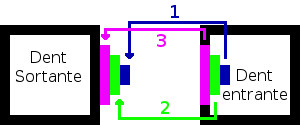
\includegraphics{dents}
\end{figure}

Nous avons créé une fonction \variable{bords} qui permet de créer les dents sur chaque côté des pièces. Cette fonction va simplement parcourir le tableaux des pièces du puzzle et appeler les fonctions \variable{bordsVertic} et \variable{bordsHoriz}. Ces dernières vont créer une dent entrante dans une pièce et une dent sortante dans l'autre. Les deux pièces passées en paramètre de ces fonctions doivent donc être côte à côte (la première dessus la deuxième pour \variable{bordsVertic} et la première à gauche de la deuxième pour \variable{bordsHoriz}).

Pour pouvoir ajouter des dents sortantes aux pièces, nous avons agrandi la taille de leur image, en placant tout autour de l'image visible un contour transparent (de largeur 1/4 de la taille de l'image visible). Ainsi, on va pouvoir changer la couleur de certains pixels transparents pour afficher une dent sortante. Pour afficher une dent entrante, il suffira de rendre certains pixels transparents.

Voici comment nous procédons pour créer une dent (ici, une dent sortante à gauche et donc entrante à droite mais le principe est identique pour les autres cas de figure) : nous copions le pixel qui est au centre de l'image de droite (verticalement) et qui est horizontalement à 1/2 de la taille de l'image visible (la bordure faisant 1/4 et on veut le pixel à la pointe du triangle), et nous le plaçons sur l'image de gauche au milieu verticalement et au dernier pixel de l'image horizontalement. Le pixel à droite sera défini transparent pour créer la dent entrante. Nous continuons ainsi de suite, mais avec 3 pixels, puis 5... jusqu'à obtenir un triangle.

%////////////////////////////////////////////////////////////////////////////////
%///////////////////////////DEUXIEME CHAPITRE THEO //////////////////
%//////////////////////////////////////////////////////////////////////////////

\newpage
\subsection{Ergonomie}

Dans cette partie nous parlerons de l'ergonomie du jeu.
\subsubsection{Placement des pièces}
Tout d'abord parlons du placement des pièces.
Pour placer les pièces nous avons procéder en différentes étapes. Dans un premier temps nous avons utilisé 4 booléens : 
\begin{lstlisting}
// Si il y a eu un clic (donc si on a une piece en main)
boolean pieceTenue = false;
// Si le tour est fini
boolean finDuCoup = false;
// Si on veut changer de puzzle
boolean relancer = false;
// Passe a true si il y a un clic (n'importe lequel)
 boolean unClic;
\end{lstlisting}

Ainsi, nous pouvons vérifier quand le clic de la souris est utilisée. 
Pour ce faire, on met à jour l'état de la souris à chaque tour de boucle. On regarde si il s'agit d'un clic gauche et on vérifie que la pièce est bien en main grâce au booléen \variable{pieceTenue}. Si ces conditions sont réunies alors le booléen \variable{pieceTenue} reste a \variable{true} pour que l'utilisateur puisse tenir la pièce jusqu'au prochain clic. Ensuite pour placer la pièce il faut un second clic gauche de la part de  l'utilisateur.
Pour que l'utilisateur puisse placer la pièce il faut qu'on vérifie que le curseur de la souris se trouve bien au dessus de la grille destinée au puzzle et que la case en dessous du curseur soit libre. Une fois que la pièce est posée le tour est fini et le booléen \variable{pieceTenue} passe à faux pour indiquer que l'utilisateur à relâché la pièce.

\subsubsection{Boutons}
Dans un second temps nous parlerons des boutons présent dans le menu. 
Chaque bouton est situé sous le puzzle.  Pour chacun d'eux on peut savoir si il y a clic ou non (voir figure \no\ref{Fonction estSurBouton}).

\begin{figure}[hpt]
	\center
	\caption{\label{Fonction estSurBouton} Fonction estSurBouton}
\begin{lstlisting}
public static boolean estSurBouton(Bouton bt)
{
    boolean estDessus = false;

    // Si la position du curseur est dans le rectangle du bouton...
    if(EcranGraphique.getMouseX() >= bt.x && EcranGraphique.getMouseX() <= bt.x + bt.larg && EcranGraphique.getMouseY() >= bt.y && EcranGraphique.getMouseY() <= bt.y + bt.haut)
        estDessus = true;

    return estDessus;
}
\end{lstlisting}
\end{figure}

Par ailleurs, nous avons utilisé la fonction drawBouton() pour créer les boutons. Chaque bouton est initialisé comme ceci :

\begin{lstlisting}
// Tout d'abord on cree un nouveau bouton
pzl.mn.relanc = new Bouton(); 
// Ensuite on lui donne un nom 
pzl.mn.relanc.label = "Autre puzzle";
// On lui indique ou celui est place en abscisse 
pzl.mn.relanc.x = x1 + 10;
// On lui indique ou celui est place en ordonnee
pzl.mn.relanc.y = y1 + 480 + 20;
// On lui indique ca largeur
pzl.mn.relanc.larg = 10 * pzl.mn.relanc.label.length();
// On lui indique ca hauteur
pzl.mn.relanc.haut = 25;
\end{lstlisting}

Nous procédons pour chaque bonton du menu comme ci dessus, en redéfinissant à chaque fois ce qu'il y a entre les lignes de codes entre les commentaires. Nous pouvons faire cela car nous avons créé le type agrégé nécessaire à la résolution de ce problème (comment afficher un bouton). Le type agrégé est celui présenté dans la figure \no\ref{Type agrégé Bouton}.

\begin{figure}[hpt]
	\center
	\caption{\label{Type agrégé Bouton} Type agrégé Bouton}
\begin{lstlisting}
static class Bouton
{
    // Position en X du bouton dans la fenetre /
    int x;
    // Position en Y du bouton dans la fenetre /
    int y;
    // Largeur du bouton 
    int larg;
    //Longueur du bouton /
    int haut;
    //Texte a afficher sur le bouton 
    String label;
    //Bouton survole ou non 
    boolean survol = false;
    //Bouton appuye ou non 
    boolean appui = false;
} 
\end{lstlisting}
\end{figure}

Comme nous pouvons le voir dans le type agrégé, nous avons utilisé un booléen \variable{survol}. En effet nous avons utilisé ce booléen pour un aspect fonctionnel du jeu : lorsque le joueur survolera un bouton, alors celui ci changera de couleur, et affichera un message à sa droite qui aidera le joueur à appréhender le jeu. Nous avons fait de même avec le clic sur le bouton : lorsque le joueur clic que le bouton, celui ci reste coloré d'une autre couleur afin que le joueur puisse connaître le mode de jeu dans lequel il joue actuellement.
 
\subsubsection{Gestion des clics}

Nous avons mis en place un système de clic. Pour ce faire nous avons utilisé le type agrégé \variable{Souris} : 

\begin{lstlisting}
static class Souris
{
    /** Position du curseur **/
    Position2D pos;
    /** Booleen qui indique si le clic droit est appuye **/
    boolean clicDroit = false;
    /** Boolean qui indique si le clic gauche est appuye **/
    boolean clicGauche = false;
}
\end{lstlisting}

Celui ci est à été extrêmement utile pour le système de gestion des clics. En effet, 
nous avons utilisé la fonction \variable{attendClic} qui retourne un booléen \variable{ret}. Dans cette fonction il est question de savoir quel bouton de la souris est pressé. Pour ce faire nous avons utilisé \variable{EcranGraphique.getMouseState()} et testé grâce à des conditions si le bouton pressé de la souris était égal à 0, 1 ou 3. Ces chiffres indiquent si 0 boutons sont pressés, si c'est le clic gauche, si c'est le clic droit. Cependant on fait également : 
\begin{lstlisting}
if(!souris.clicGauche)
{
    ret = true;
    souris.clicGauche = true;
}
\end{lstlisting}

Afin de ne renvoyer vrai que la première fois qu'on voit le clic. Nous procédons de même pour le clic droit.

Voila comment nous avons simplifié le système de clic pour le faire correspondre à notre besoin pour ce jeu (nous n'avons pas besoin, par exemple, de savoir combien de temps le joueur clique).

%///////////////////////////////////////////////////////////////////////////////
%///////////////////////////TROISIEME CHAPITRE THEO/////////////////
%//////////////////////////////////////////////////////////////////////////////

\newpage
\subsection{Gameplay}

Cette partie comprendra des explications concernant le gameplay. 

\subsubsection{Nombres de coups et temps}

Nous avons réalisé un chronomètre permettant de connaitre le temps que le joueur a pris pour résoudre le puzzle. 
Pour cela, nous avons utilisé la variable \variable{pzl.temps} que nous définissons grâce à la fonction de java pour récupérer l'heure actuelle en millisecondes :\variable{ java.lang.System.currentTimeMillis()}. 
Ensuite, nous avons juste à reprendre l'heure à laquelle le puzzle à été reconstitué et y soustraire pzl.temps qui à été initialisé lors de l'initialisation du puzzle et aussi à chaque nouveau puzzle.
Cependant il nous a fallu convertir les millisecondes en secondes afin de faciliter la lecture pour l'utilisateur. De plus, nous avons créé une fonction permettant de n'afficher que le nécessaire : figure \no\ref{Fonction tempsResolution}.

\begin{figure}[hpt]
	\center
	\caption{\label{Fonction tempsResolution} Fonction tempsResolution}
\begin{lstlisting}
public static String tempsResolution(long nbSecondes)
{
    String msgFin;
    long heure   = nbSecondes / 60 / 60;
    long minute  = nbSecondes  / 60  % 60;
    long seconde = nbSecondes  % 60;

    msgFin = "et tu as mis ";
    if (heure <=0 && minute <=0)
    {
        msgFin = msgFin + seconde + " seconde(s).";
    }
    if (minute >= 1 && heure <= 0  )
    {
        msgFin = msgFin + minute + " minute(s) " + seconde + " seconde(s).";
    }
    if ( heure >= 1 && minute >=1 )
    {
        msgFin = msgFin + heure +" heure(s) et " + minute +" minute(s) et "  + seconde +" seconde(s).";
    }
    return msgFin;
}
\end{lstlisting}
\end{figure}

Pour le nombre de coups, nous avons compté tout les tours en les stockant dans une variable \variable{nbCoups} que nous augmentons de 1 à chaque fois qu'un tour est terminé (à chaque fois qu'on quitte la fonction \variable{jouerCoup}. Nous vérifions aussi si le puzzle est fini : lorsque le puzzle est reconstitué nous n'avons qu'à appeler la variable et nous connaissons alors le nombre de coups qu'il a fallu au joueur pour résoudre le puzzle. A noter que la rotation de pièce compte comme un coup.

\subsubsection{Nouvelle partie}

Le joueur peut a la fin d'une partie relancer une partie en cliquant n'importe où. Pour que le puzzle se relance nous avons créé un booléen \variable{relancer} qui permet de savoir si l'utilisateur veut un autre puzzle ou non. Si l'utilisateur veut un nouveau puzzle, alors on réinitialise tout, l'image, le chronomètre le nombre de coups. En fait, on test la condition de relancer jusqu'à ce que celui ci passe à vrai. Dans ce cas tout est réinitialisé. 

\subsubsection{Condition de fin}

À la fin du jeu, le joueur doit savoir si celui-ci à résolu le puzzle ou non. Pour cela, nous avons créé la fonction en figure \no\ref{Fonction  estReconstitue}.

\begin{figure}[hpt]
	\center
	\caption{\label{Fonction  estReconstitue} Fonction  estReconstitue}
\begin{lstlisting}
public static boolean estReconstitue(PuzzleJeu pzl)
{
    int i = 0;
    int j;
    boolean reconstituee = true;

    while(i < nbPiecesX && reconstituee) // Tant qu'on n'a pas trouve de case non placee
    {
        j = 0; // On remet a zero j pour compter a partir de zero a chaque tour
        while(j < nbPiecesY && reconstituee) // Tant qu'on n'a pas trouve de case non placee
        {
            if(!pzl.pieces[i][j].placee || pzl.pieces[i][j].rotation != 0)
            {
                reconstituee = false;
            }
            j++; // Incrementation de j a chaque tour de la boucle interieure
        }
        i++; // Incrementation de i a chaque tour de la premiere boucle
    }

    return reconstituee;
}
\end{lstlisting}
\end{figure}

Tant que la fonction ci dessus retourne \variable{false} alors le puzzle n'est pas résolu. Finalement, on teste pour chaque pièce si elle est à la bonne place. Et si c'est le cas, alors la fonction retourne \variable{true}. 





%/////////////////////////////////////////////////////////////////////////////////
%///////////////////////////QUATRIEME CHAPITRE EMILE/////////////////
%//////////////////////////////////////////////////////////////////////////////

\subsection{Affichage et déplacements}

Cette partie décrira comment nous avons résolu la question de l'affichage et du déplacement des pièces.

\subsubsection{Déplacement des pièces}

Nous avons décidé que la pièce suivrait le curseur lorsqu'elle est sélectionnée. Pour cela, nous vérifions (dans la fonction \variable{jouerCoup} que l'utilisateur effectue un clic gauche sur une pièce et qu'il n'y avait pas de pièces tenue à ce moment. Si l'utilisateur avait dans la main une pièce, elle sera posée par cette action. Donc après un clic sur une pièce, la pièce en question va suivre le curseur. En effet, cette pièce est identifiée par \variable{pzl.caseChoisie} avec \variable{pzl} notre variable \variable{PuzzleJeu} contenant le puzzle entier et \variable{caseChoisie} qui est une position : celle de la case tenue par l'utilisateur.

À chaque tour de boucle, nous mettons à jour la position de la pièce correspondant à \variable{caseChoisie} (uniquement si caseChoisie est valide : si aucune case n'est tenue, \variable{caseChoisie.x = -1} et \variable{caseChoisie.y = -1}. Le curseur doit se trouver au centre de l'image, la position sera donc affectée en conséquence.

Enfin, dans l'affichage, cette case devra être affichée après les autres pour ne pas qu'elle soit visuellement en dessous d'une autre lorsqu'on la déplace (et qu'on puisse ainsi déduire sa véritable position dans la grille).

\subsubsection{Affichage}

Nous avons décidé de créer une fonction affichage qui gérera tout l'affichage du puzzle. Pour cela, nous lui envoyons notre variable principale \variable{PuzzleJeu pzl}.

La première étape est de nétoyer l'écran, c'est à dire d'exécuter : 
\begin{lstlisting}
EcranGraphique.clear();
\end{lstlisting}

Ensuite, nous dessinons la grille : des lignes horizontales et des lignes verticales du même nombre de pixels que l'image (en largeur ou hauteur), et nous traçons également les instructions du jeu : quelques règles.

Vient ensuite l'affichage des pièces : l'image contenue dans celles-ci est tracée (image qui a pu être tournée préalablement), mais on prend soin de ne pas tracer l'image tenue (si il y en a une). Nous ne dessinons qu'ensuite l'image tenue, afin qu'elle soit affichée au dessus des autres.

Nous traçons ensuite le texte de réussite si le puzzle est fini, puis nous affichons le menu (avec ses différents boutons) et des textes d'aide pour chaque bouton.

On termine la fonction en affichant le tout à l'écran. 

%/////////////////////////////////////////////////////////////////////////////////
%///////////////////////////INDEX/////////////////////////////////////////////
%//////////////////////////////////////////////////////////////////////////////

\newpage


\end{document}
